% Definicoes do \documentclass

\documentclass[ppginf, pep]{esinucpel}

\usepackage[utf8]{inputenc}
\usepackage[T1]{fontenc}
\usepackage{graphicx}
\usepackage{float}
\usepackage{hyperref}
\usepackage{listings}
\usepackage{color}

\graphicspath{ {images/} }

% Code blocks
\definecolor{dkgreen}{rgb}{0,0.6,0}
\definecolor{gray}{rgb}{0.5,0.5,0.5}
\definecolor{mauve}{rgb}{0.58,0,0.82}
\definecolor{lightgray}{rgb}{.9,.9,.9}
\definecolor{darkgray}{rgb}{.4,.4,.4}
\definecolor{purple}{rgb}{0.65, 0.12, 0.82}
\lstdefinelanguage{JavaScript}{
  keywords={break, case, catch, continue, debugger, default, delete, do, else, false, finally, for, function, if, in, instanceof, new, null, return, switch, this, throw, true, try, typeof, var, void, while, with},
  morecomment=[l]{//},
  morecomment=[s]{/*}{*/},
  morestring=[b]',
  morestring=[b]",
  ndkeywords={class, export, boolean, throw, implements, import, this},
  keywordstyle=\color{blue}\bfseries,
  ndkeywordstyle=\color{darkgray}\bfseries,
  identifierstyle=\color{black},
  commentstyle=\color{purple}\ttfamily,
  stringstyle=\color{red}\ttfamily,
  sensitive=true
}

\lstset{frame=tb,
  language=JavaScript,
  aboveskip=3mm,
  belowskip=3mm,
  showstringspaces=false,
  columns=flexible,
  basicstyle={\small\ttfamily},
  numbers=none,
  numberstyle=\tiny\color{gray},
  keywordstyle=\color{blue},
  commentstyle=\color{dkgreen},
  stringstyle=\color{mauve},
  breaklines=true,
  breakatwhitespace=true,
  tabsize=4
}

% Inline code
\newcommand{\code}[1]{\texttt{#1}}



%\usepackage[acronym]{glossaries}

% Abreviaturas:
%\newacronym{tc39}{TC39}{Technical Committee 39}

\title{Harmonic: O Próximo Gerador de Sites Estáticos}

\author{Matté}{Fabrício da Silva}
\advisor[Prof.]{Rodrigues}{Sérgio Luis}
% \coadvisor[Prof.~Dr.]{Aguiar}{Marilton Sanchotene de}
% \collaborator[Prof.~Dr.]{Aguiar}{Marilton Sanchotene de}


\keyword{Gerador de Sites Estáticos}
\keyword{Node.js}
\keyword{ECMAScript 2015}

%\makeglossaries
\begin{document}

%\renewcommand{\advisorname}{Orientadora}           %descomente caso tenhas orientadora
%\renewcommand{\coadvisorname}{Co-orientadora}      %descomente caso tenhas co-orientadora

\maketitle
\sloppy

% Glossário de abreviaturas
%\printglossary[type=\acronymtype,title=Lista de abreviaturas e siglas]

% Sumário
\tableofcontents

% Resumo em Portugues (no maximo 250 palavras)
\begin{abstract}

O projeto Harmonic tem por objetivo desenvolver um gerador de sites estáticos, utilizando como base a plataforma Node.js juntamente com os recursos mais recentes da linguagem JavaScript que foram especificados no padrão ECMAScript 2015 \cite{es2015}, o qual foi finalizado e oficializado como padrão da linguagem JavaScript em Junho de 2015. O compilador Babel é utilizado para atingir este objetivo, o qual transforma código que utiliza recursos de especificações recentes e futuras do JavaScript em código que pode ser executado nos motores JavaScript atuais.

O Harmonic roda sobre a plataforma Node.js, que é, de forma resumida, um motor JavaScript combinado com servidor Web, que permite execução do mesmo código JavaScript em todas as principais plataformas (Windows, Linux, Mac), sem possuir as restrições de segurança comumente encontradas no ambiente de navegadores. Ou seja, o código JavaScript executado pelo Node.js tem acesso completo ao sistema de arquivos e rede da máquina hospedeira, e esta é uma das principais capacidades do Node.js das quais o Harmonic utiliza para gerar sites estáticos.

\end{abstract}

\begin{englishabstract}{Harmonic: The Next Static Site Generator}{Static Site Generator, Node.js, ECMAScript 2015}

The Harmonic project aims to develop a static site generator, using the Node.js platform as its base together with the most recent JavaScript features that have been specified in the ECMAScript 2015 standard \cite{es2015}, which was completed and officially published as the JavaScript language standard in June 2015. The Babel compiler is utilized to achieve this goal, which transforms code that uses features from the most recent and future JavaScript specifications into code that can be run in the current JavaScript engines.

Harmonic runs on the Node.js platform, which is, basically, a JavaScript engine combined with a Web server, which enables the same JavaScript code to run in all the major platforms (Windows, Linux, Mac), having none of the security restrictions often found in the browser environment. That is, the JavaScript code run by Node.js has full access to the host machine's file system and network, and this is one of the main Node.js capabilities of which Harmonic uses to generate static sites.

\end{englishabstract}

\chapter{Introdução}

O projeto Harmonic trata-se de um gerador de sites estáticos. Ou seja, é um programa capaz de gerar uma estrutura de pastas e \emph{arquivos fonte} onde o usuário pode criar e gerenciar o conteúdo de seu site, além de poder instalar, criar ou personalizar \emph{temas}, que são grupos de arquivos de \textit{template}.

O Harmonic pode ser instalado de forma gratuita pelo gerenciador de pacotes \emph{npm} \cite{npm}. Os temas do Harmonic geralmente são disponibilizados através de pacotes também distribuídos pelo npm, mas o usuário também possui a opção de criar temas privados sem a necessidade de publicá-los no npm, assim como não compartilhá-los com o público.

Outra característica importante do projeto Harmonic é que todo seu desenvolvimento se dá de forma aberta, tendo não apenas todo seu \emph{código fonte} acessível publicamente em um repositório hospedado no serviço do \href{https://github.com/}{GitHub}, mas também todas discussões, reportagem de problemas, tomadas de decisões e governança do projeto também se dá de forma aberta no próprio \textit{issue tracking system} do GitHub, que é utilizado como uma espécie de sistema de gerenciamento do projeto.

O projeto Harmonic está sendo escrito sobre a plataforma \emph{Node.js}, que possibilita a execução de programas escritos na linguagem de programação JavaScript nos principais Sistemas Operacionais (Windows, OS X e várias distribuições de Linux). Desta forma, todo projeto é escrito em uma linguagem de programação fácil de escrever e contribuir, além de não possuir limitações comumente encontradas no ambiente de um \textit{browser}.

O foco principal deste projeto está na ergonomia do usuário e simplicidade de ser utilizado. O usuário está sempre em primeiro plano. Recursos como recompilar arquivos automaticamente ao serem modificados assim como recarregar o site em desenvolvimento automaticamente quando há mudanças, além da excelente performance da ferramenta e a simplicidade da interface de linha de comando, facilitam a vida do usuário e o deixam mais produtivo.

Um dos objetivos complementares deste projeto é aprender, explorar e demonstrar os novos recursos oferecidos pela linguagem JavaScript, como aqueles introduzidos nas novas edições da especificação ECMAScript, assim como nas propostas que estão em andamento no processo de padronização do TC39 (Technical Committee 39, grupo responsável pela evolução da linguagem JavaScript) da associação \textit{ECMA International}. % TODO: TC39 provavelmente deveria ser marcado como acrônimo

Na próxima seção veremos um pouco mais sobre o tema e metodologia do projeto. % TODO: listar todos capítulos seguintes

% TODO: falar um pouco mais sobre a interface de linha de comando, talvez?

% TODO: esta seção carece de referências.

\section{Justificativa}

\section{Objetivos}

O objetivo geral deste trabalho é explorar a área de geradores de sites estáticos, desenvolvendo um novo gerador de sites estáticos com recursos inovadores e fazendo uso das últimas tecnologias relacionadas à linguagem JavaScript.

Os objetivos específicos são:
\begin{itemize}
	
	\item estudar e aprofundar a metodologia de criação de sites estáticos;
	\item estudar os recursos das próxima(s) versão(ões) do JavaScript (ECMAScript 2015 e além);
	\item estudar a plataforma Node.js;
    \item criar um gerador de sites estáticos com recursos que os demais ainda não possuem;

\end{itemize}

\chapter{Fundamentação Teórica}

A proposta dos sites estáticos é um tema bem popular atualmente, tendo mais de 435 geradores de sites estáticos já existentes. \cite{staticsitegenerators}

Ao contrário dos sites dinâmicos, que requisitam banco de dados e executam lógica no servidor para cada requisição, todo o conteúdo de um site estático é gerado instantaneamente antes de qualquer acesso por parte de usuários, assim podendo ser hospedado em um servidor que não necessita de banco de dados nem suporte a nenhuma linguagem de programação.

Além disto, como diz David Walsh, sites estáticos são muito mais rápidos que os dinâmicos, pois todo processamento de conteúdo já foi realizado no momento da geração do site estático e não a cada requisição como nos sites dinâmicos. Outro ponto é a segurança, sites estáticos são extremamente mais seguros que os dinâmicos pois não possuem lógica de programação no servidor, o que os torna a prova de falhas de segurança na programação do lado do servidor. \cite{dwb}

Praticamente todos geradores de sites suportam a escrita de conteúdo através da linguagem de marcação Markdown, que é basicamente uma versão simplificada, mais fácil de escrever e ler do que a linguagem de marcação HTML. Markdown é uma ferramenta de conversão de texto para HTML para escritores Web  \cite{markdown}. O projeto Harmonic também suporta a linguagem de marcação Markdown e o converte para HTML na momento da geração do conteúdo.

O projeto Harmonic é desenvolvido sobre a plataforma Node.js, que suporta todos os principais sistemas operacionais (OS X, Linux, Solaris, FreeBSD, OpenBSD, Windows, webOS, NonStop OS) nos permitindo executar o mesmo código em todas estas plataformas. A plataforma Node.js executa código JavaScript, que é uma linguagem de programação leve e bem simplificada \cite{mdn_js_intro}, assim facilitando no desenvolvimento. O Node.js também possui mais de 250.000 pacotes públicos publicados no registro de pacotes mais popular, npm \cite{npm}, o que torna o desenvolvimento muito mais ágil permitindo reutilizar "blocos de construção" para construir sistemas maiores. \cite{micromodules}

\chapter{Metodologia de Pesquisa}

sub-capítulo: experiência própria

sub-capítulo: Sistemas semelhantes

Vejamos uma comparação entre os Sistemas Semelhantes.

\chapter{Modelagem do Sistema}

Após especificar o que o sistema deveria possuir, passou-se à etapa de criação dos diagramas para identificar como deve ser o processo de comunicação entre os vários componentes do sistema e a utilização do UML facilitou a modelagem do software.

UML é uma linguagem de modelagem que auxilia os desenvolvedores na montagem dos requisitos e do comportamento dos processos no sistema, também atua na descoberta de possíveis necessidades físicas que possam surgir na implementação de uma determinada ferramenta. \cite{uml}

UML é uma metodologia que disponibiliza diversas maneiras para analisar uma determinada questão e neste projeto será utilizado uma abordagem orientada a objetos, que auxilia na reutilização de métodos ou atributos, melhorando o desenvolvimento e a manutenção do sistema. Os itens a seguir apresentam diagramas para facilitar o entendimento do leitor.

\section{Diagrama de Sequência}

Foram criados diagramas de sequência pois estes ajudam a planejar o fluxo de informações e operações a serem realizadas pelas rotinas do sistema. O diagrama de sequência da execução do site estático, que é uma das principais funcionalidades do Harmonic, pode ser conferido na figura \ref{fig:sequencia}.

\begin{figure}[H]
    \centering
    \caption{Diagrama de sequência da execução de um site estático do Harmonic.}
    \vspace{5pt}
    \includegraphics[width=\textwidth]{sequencia}
    \\Fonte: Elaborado pelo autor.
    \label{fig:sequencia}
\end{figure}

\section{Diagrama de Casos de Uso}

Foi criado um diagrama de casos de uso pois este facilita mapear as funcionalidades que o sistema deve desempenhar assim como as relações entre elas. O diagrama de casos de uso do Harmonic pode ser conferido na figura \ref{fig:casos_de_uso}.

\begin{figure}[H]
    \centering
    \caption{Diagrama de casos de uso do Harmonic.}
    \vspace{5pt}
    \includegraphics[width=\textwidth]{casos-de-uso}
    \\Fonte: Elaborado pelo autor.
    \label{fig:casos_de_uso}
\end{figure}

\chapter{Tecnologias e Ferramentas Utilizadas}

\section{JavaScript}

JavaScript é uma linguagem de programação orientada a objetos multiplataforma. Dentro de um ambiente hospedeiro (por exemplo, um navegador web), JavaScript pode ser conectado aos objetos de seu ambiente para prover controle sobre eles. O padrão oficial da linguagem JavaScript é o ECMAScript. \cite{mdn_js_intro}

O JavaScript obteve uma evolução significativa nos últimos anos, tornando-se assim uma das linguagens de propósito geral mais utilizadas no mundo. É mais conhecida como a linguagem incorporada aos navegadores Web, mas também houve um grande crescimento em sua adoção por parte de servidores e aplicações embarcadas. \cite{es2015}

O projeto Harmonic escolheu esta linguagem de programação devido a sua ampla aceitação no mercado e rápida evolução, além de esta linguagem ser relativamente simples e fácil de trabalhar, contendo centenas de milhares de pacotes comunitários que facilitam no desenvolvimento de praticamente qualquer sistema.

\section{Node.js}

Node.js é uma plataforma de código fonte aberto que permite construir aplicações em rede utilizando a linguagem JavaScript. Node.js é construído em cima do V8, uma máquina virtual JavaScript moderna que também é utilizada pelo navagedor Web Google Chrome. \cite{instant_nodejs_starter:03}

Node.js é um \textit{runtime} JavaScript assíncrono orientado a eventos. \cite{nodejs} Isto que dizer que o Node.js pode ser considerado uma plataforma que combina um motor JavaScript com acesso a recursos do sistema operacional hospedeiro.

A plataforma Node.js roda diretamente sobre o sistema operacional, com isto é possível executar código JavaScript completamente fora do ambiente de um navegador Web. Assim sendo, o Node.js não interage com uma página da Web diretamente, mas sim com os recursos do computador hospedeiro. Por exemplo, o Node.js pode receber e realizar requisições HTTP, ler e escrever no sistema de arquivos, e se comunicar com outros processos, \textit{sockets} e \textit{drivers} do sistema operacional. \cite{javaworld}

Todo o projeto Harmonic é construído sobre a plataforma Node.js, que realiza toda lógica de negócios e leitura e escritas ao sistema de arquivos do usuário.

\section{npm}

O npm é o gerenciador de pacotes padrão da plataforma Node.js, contando com mais de 250.000 pacotes publicados \cite{npm} e provendo mais de um bilhão de instalações de pacotes semanalmente \cite{npm_packages}.

O projeto Harmonic escolheu o npm como sua plataforma de distribuição e gerenciador de dependências devido ao seu fácil acesso, altíssima resiliência e ubiquidade na comunidade Node.js.

\section{JSON}

JSON (JavaScript Object Notation) é um formato de troca de informações eficiente. É fácil de ler e escrever manualmente. É fácil de analisar e gerar por computadores, assim como ler e escrever por desenvolvedores. \cite{json}

O projeto Harmonic escolheu o formato JSON para o armazenamento de configurações, pois este formato facilita a operação dos dados tanto pelo sistema quanto pelo usuário final.

\section{Markdown}

\section{gulp}

\section{Babel}

\section{BrowserSync}

\chapter{Descrição do Sistema}

\section{Estrutura do projeto}

O Harmonic divide-se em vários módulos, sendo eles: criação de um novo site estático, configuração do site estático, criação de \textit{posts} e páginas, geração do site estático e execução do site estático, além do módulo de ajuda.

Assim como a maioria dos pacotes, bibliotecas e ferramentas escritas sobre a plataforma Node.js, o Harmonic está publicado no registro de pacotes do npm e pode ser instalado através do gerenciador de pacotes que faz parte da instalação padrão do Node.js, ou seja, através da ferramenta de linha de comando do npm.

E, similarmente a outros geradores de sites estáticos, o Harmonic conta uma ferramenta de linha de comando que pode ser utilizada para criar um novo site estático, adicionar conteúdo ao mesmo, compilar o site estático e visualizá-lo no navegador.

\section{Módulo de criação de um novo site estático}

O Harmonic permite a criação de novos sites estáticos através do comando \code{harmonic init}. Este comando gera uma estrutura padrão de pastas e arquivos, onde são guardados todos arquivos fontes do site estático.

O comando \code{harmonic init} realiza uma série de questionamentos sobre as configurações e personalizações que o site deve possuir (conforme pode ser conferido na figura \ref{fig:harmonic_init}), então escreve estas configurações no arquivo de configuração do site estático \code{harmonic.json}. O usuário pode futuramente modificar estas configurações utilizando o comando \code{harmonic config} ou editando o arquivo de configuração \code{harmonic.json} em qualquer editor de texto, já que o arquivo de configuração nada mais é do que um arquivo de texto no formato \emph{JSON}.

\begin{figure}[H]
    \centering
    \caption{Exemplo do comando "harmonic init".}
    \vspace{5pt}
    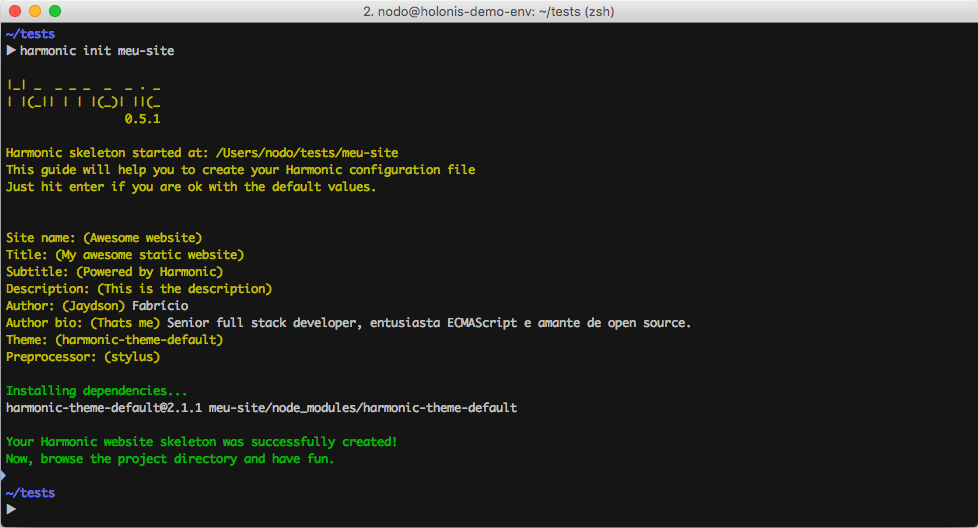
\includegraphics[width=.85\textwidth]{harmonic_init}
    \\Fonte: Elaborado pelo autor.
    \label{fig:harmonic_init}
\end{figure}

\section{Configurações disponíveis}

A FAZER

\section{Criação de novos \textit{posts}}

O usuário pode criar novos \textit{posts} utilizando o comando \code{harmonic new\underline{ }post "\textless TÍTULO DO POST\textgreater"}, que criará um arquivo \emph{Markdown} dentro da pasta fonte de \textit{posts} de cada linguagem que o site estático suporta.

\subsection{Meta-informações e configurações de \textit{posts}}

Cada arquivo fonte de \textit{post} possui um cabeçalho de meta-informações, no formato de um comentário HTML contendo pares de chaves e valores, como pode ser visto na figura \ref{fig:post_header}.

\begin{figure}[H]
    \centering
    \caption{Exemplo de cabeçalho de meta-informações de um \textit{post} do Harmonic.}
    
    \lstset{language=HTML}
    \begin{lstlisting}
    <!--
    layout: post
    title: JavaScript iterables and iterators
    date: 2015-09-15T04:06:02.428Z
    comments: true
    published: true
    keywords: iterables, iterators, ES2015
    description: Understanding JavaScript ES2015 Iterables and Iterators
    categories: iterables, iterators, ES2015, articles
    authorName: UltCombo
    authorLink: https://twitter.com/Ult_Combo
    authorDescription: Full Stack developer, ECMAScript enthusiast, open source lover.
    authorPicture: https://s.gravatar.com/avatar/326fba1c2980ce0073f6b212acf71ea0
    -->
    \end{lstlisting}
    
    Fonte: Elaborado pelo autor.
    \label{fig:post_header}
\end{figure}

\begin{itemize}
	\item \textbf{\code{layout}}: nome do arquivo HTML do tema selecionado a ser utilizado na renderização deste \textit{post}. O valor padrão é \code{post}.
	\item \textbf{\code{title}}: título do \textit{post}.
	\item \textbf{\code{date}}: data de publicação deste \textit{post}. Pode ser utilizado para agendar uma publicação futura.
	\item \textbf{\code{comments}}: Um valor booleano indicando se o \textit{post} deve permitir comentários ou não. Note que nem todos temas suportam comentários. O valor padrão é \code{true}.
	\item \textbf{\code{published}}: Um valor booleano indicando se o \textit{post} está publicado ou não. Pode ser utilizado para despublicar ou ocultar o \textit{post}. O valor padrão é \code{true}.
	\item \textbf{\code{keywords}}: Palavras-chave descrevendo o \textit{post}.
	\item \textbf{\code{description}}: Descrição resumida do \textit{post}.
	\item \textbf{\code{categories}}: Lista de categorias a qual o \textit{post} pertence, separadas por vírgulas. Você pode especificar qualquer nome de categoria, se a mesma não existir ela será criada.
	\item \textbf{\code{authorName}}: Nome do autor do \textit{post}.
	\item \textbf{\code{authorDescription}}: Biografia resumida do autor do \textit{post}.
	\item \textbf{\code{authorPicture}}: Endereço URL para a foto de perfil do autor do \textit{post}.
\end{itemize}

\section{Geração do site estático}

Para consumir o conteúdo do site é necessário primeiro gerar o site estático, que é basicamente um processo de compilação. Para isso, pode-se utilizar o comando \code{harmonic build}, que gera o site estático a partir dos arquivos fontes (configurações, tema ativo e arquivos Markdown) do seu site Harmonic, assim gerando arquivos HTML, CSS e JS como saída.

Com estes arquivos, então, é possível abrir o arquivo \code{index.html} em seu navegador de preferência e navegar pelo site estático.

Note que qualquer edição ou mudança realizada nos arquivos fontes do site, incluindo edição de \textit{posts} e alteração de configurações, requer uma nova compilação para que as mudanças sejam refletidas nos arquivos compilados.

\section{Execução do site estático}

O Harmonic também dispõe do comando \code{harmonic run}, que além de realizar o mesmo processo de compilação que o \code{harmonic build}, também inicia um servidor local para servir os arquivos estáticos e automaticamente abre o site estático no navegador padrão do sistema. Este é o método indicado para pre-visualização de seu site estático, pois os navegadores frequentemente bloqueiam vários recursos JavaScript ao acessar os arquivos estáticos diretamente do disco sem um servidor envolvido no processo, o que pode afetar a funcionalidade do site caso você abra os arquivos diretamente no navegador como descrito na seção anterior.

Além disso, o comando \code{harmonic run} também conta com um recurso de auto-geração de site e auto-recarregamento do navegador ("\textit{live-reload}") sempre que ocorrerem alterações nos arquivos fontes do site, assim proporcionando uma experiência de criação de conteúdos otimizada e muito mais prática e eficiente.

Por padrão, o comando \code{harmonic run} inicia um servidor local na porta \code{9356}, e abre o site no navegador padrão do sistema automaticamente. É possível customizar estes recursos, passando a porta desejada como primeiro parâmetro do comando (exemplo: \code{harmonic run 8080}), assim como desabilitar a função de abrir o site automaticamente passando a \textit{flag} \code{--no-open}.

\chapter{Considerações Finais}

\section{Resultados obtidos e discussões}

\section{Trabalhos Futuros}

\subsection{Plugins}

A FAZER

\subsection{Melhorias no desenvolvimento de temas}

A FAZER

% \chapter{Exemplo de código JavaScript}

% (capítulo temporário, por enquanto apenas testando o syntax highlighter)

% \lstset{language=JavaScript}
% \begin{lstlisting}
% // Hello.js
% function foo(arg) {
%	alert(1);
% }
% \end{lstlisting}

% Exemplo puxando o código fonte de um arquivo separado:
% \lstinputlisting[breaklines]{source.js}


%É crescente o uso de tecnologia na prestação de serviços de saúde. As atividades de segunda opinião, monitoramento de pacientes, telediagnóstico remoto entre outras são atividades utilizadas mediante uma infraestrutura de rede, realizadas por profissionais conectados em outro centro médico distante da localidade onde o paciente está sendo examinado.
%Estes cenários são interessantes pois reduzem custos com relação ao deslocamento dos profissionais de saúde e com relação à troca de informações sobre diagnósticos. Todo o histórico de um paciente pode ser armazenado em um Prontuário Eletrônico do Paciente (PEP), e através do acesso aos dados é possível auxiliar na obtenção de um diagnóstico completo e eficaz.
%
%De acordo com o Conselho Federal de Medicina, o prontuário do paciente é um documento único constituído de um conjunto de informações, sinais e imagens registradas, geradas a partir de fatos, acontecimentos e situações sobre a saúde do paciente e a assistência a ele prestada, de caráter legal, sigiloso e científico, que possibilita a comunicação entre membros da equipe multiprofissional e a continuidade da assistência prestada ao indivíduo \cite{CFM:02}.
%
%Com a expansão das redes de comunicação, possibilitando larguras de banda superiores, comunicação sem fio e acesso através de dispositivos de menores dimensões, como Notebooks, Smartphone,  Personal Digital Assistant (PDA), entre outros, o uso de tecnologia móvel nos ambientes de saúde tornou-se um desafio possível. Através do uso de dispositivos de menores dimensões e de enlaces de comunicação sem fio e de alta velocidade, é possível se fazer acesso ao PEP, de maneira ubíqua, conforme conceito introduzido por Weiser e colegas \cite{weiser:99}.
%Segundo Weiser, através da computação ubíqua, o usuário pode ter acesso ao seu ambiente computacional a partir de qualquer lugar, em qualquer momento, de várias formas, através de  dispositivos diferentes e com as mais variadas formas de tecnologias de comunicação.
%
%Weiser e colegas \cite{weiser:99} argumentam que computadores de pequenas dimensões estarão embutidos em objetos do cotidiano do usuário, tais como livros, roupas e objetos pessoais em geral, interagindo entre si e adaptando o comportamento de suas aplicações, de acordo com informações relevantes à sua execução. Dessa forma, estes elementos seriam sensíveis ao contexto que os cercam, em busca de informações que possam aprimorar a execução de suas aplicações.
%
%Segundo Diniz ~\cite{Diniz:09} ambientes de prestação de serviços de saúde, o suporte à mobilidade é uma questão importante, tendo em vista que a mobilidade dos médicos é inerente à própria profissão. Além deste caráter nômade do médico é importante considerar que a atividade médica é bastante fragmentada, ou seja, está sujeita a interrupções durante sua execução, pois poderá realizar consultas presenciais, realizar cirurgias, visitas a pacientes, em deslocamento para sua residência ou local de trabalho, de sobreaviso em sua casa ou local de lazer, e ser interrompido por um paciente ou colega para a tomada de alguma decisão com relação à saúde de algum paciente. Da mesma forma, o médico poderá realizar uma consulta ou inclusão de dados de algum prontuário eletrônico de paciente e ser interrompido para a realização de alguma atividade de urgência. Em cada uma dessas situações, o médico poderá ter à sua disposição diferentes dispositivos, tais como Personal Computer (PC), Notebooks, Tablets, Palmtops, Smartphones, PDAs com configurações diversas e poderá fazer acesso ao sistema de informações de saúde de qualquer um deles. Também poderá ser permitido que o médico inicie a sessão usando um dispositivo, transfira-a para outro dispositivo, concluindo-a em um terceiro.
%
%Para constatar o caráter nômade e fragmentado da atividade médica, observa-se o trabalho descrito por Tentori e Favela \cite{tentori:08}. Eles realizaram um estudo de caso em um hospital público, onde observaram as práticas do corpo médico dentro do hospital. Verificou-se que os funcionários da equipe pesquisada (médicos, enfermeiros, técnicos entre outros) se movem mais de 50\% do tempo. A análise mostrou ainda que em 69\% do tempo eles estão interagindo com outras pessoas e que 26\% dessas interações envolvem dispositivos, como, por exemplo, telefones. Os funcionários gastam em média 2,5 minutos em cada interação. Também conseguiram constatar que o trabalho desempenhado é altamente fragmentado. Os médicos não gastam mais que cinco minutos conduzindo uma atividade, sem serem interrompidos. Eles também mensuraram o tempo de transição entre atividades, ou seja, o tempo decorrido entre duas atividades consecutivas, e verificaram, então, que este tempo chegava, em média, a 51 segundos. Essa fragmentação, normalmente, ocorre devido a uma necessidade de interrupção, devido a um chamado ou alguma atividade de maior urgência.
%
%Conforme pode ser observado, o cenário de aplicação desta dissertação é voltado para auxiliar os profissionais na área de saúde em sua rotina diária nos hospitais e consultórios, sobretudo no relacionamento com os pacientes, no que diz respeito ao uso de PEPs, e acompanhamento médico à distância. Considera-se um ambiente de computação ubíqua, aquele onde há diversos dispositivos computacionais (heterogêneos) nos vários locais por onde um médico passa, e o software de auxílio ao trabalho médico seja capaz de descobrir recursos computacionais disponíveis se adaptar de forma sensível a contexto e perceber o estado do paciente e do ambiente.
%
%O grupo G3PD ao qual este trabalho está sendo desenvolvido vem ultimamente pesquisando sobre computação ubíqua/pervasiva desenvolvendo serviço para um \textit{middleware} chamado de EXEHDA. Neste trabalho procuro identificar os desafios de pesquisa na área de medicina ubíqua e com os resultados a serem obtidos a perspectiva é adequar o uso dos serviços do  \textit{middleware} EXEHDA para as demandas funcionais introduzidas pela medicina ubíqua.


% \chapter{Escopo do Trabalho}

% \section{Medicina Ubíqua: Principais Demandas}

%Ambientes  de  medicina  ubíqua  são  aqueles  em  que  facilidades  tecnológicas, como dispositivos móveis e redes de comunicação sem fio, trazem novas possibilidades de acesso e interação de seus usuários, como por exemplo, o acesso das informações dos pacientes. Estas  informações  compõem  o  chamado  Prontuário Eletrônico  do  Paciente (PEP),  permitindo  que  dados  sobre  exames,  fatos  e  situações  sobre  a  saúde  de  um paciente possam  ser acessados através de múltiplos dispositivos e  redes  heterogêneas. Na medicina ubíqua podem-se  realizar acessos a PEPs com  informações consolidadas sobre os pacientes de qualquer lugar da rede, permitindo, inclusive, que haja cooperação entre profissionais independentemente do tempo e do espaço \cite {Diniz:09}.
%
%Em  particular,  ambientes  de  medicina  ubíqua  precisam  oferecer  suporte  à mobilidade  de  seus  profissionais,  tendo  em  vista  que  a  mobilidade  dos  médicos  é inerente  à  própria  profissão.  Além  desse  caráter  nômade  do  médico,  é  importante considerar  que  a  atividade  médica  é  bastante  fragmentada \cite {tentori:08}, ou seja, está sujeita a  interrupções durante sua execução, uma vez que médicos passam  pouco  tempo  em  cada  local  ou  atividade.  Dessa  forma,  mecanismos  que facilitem  a  continuidade  de  atividades  dos  profissionais,  mesmo  em  virtude  de  seus constantes deslocamentos, tendem a melhorar a produtividade dos mesmos \cite{Diniz:09} .
%
%Como já mencionado anteriormente, os médicos e colaboradores de hospitais trabalham em constante movimento. O trabalho descrito em \cite{Rodriguez:04} também se utiliza desta motivação reafirmando a necessidade de constante mudança de localização por parte destes profissionais em suas atividades diárias.
%
%A informação requerida por um especialista é dependente da sua localização. Por exemplo, o acesso aos resultados de exames laboratoriais de pacientes deve ser mais relevante quando o médico estiver perto do paciente que quando ele estiver em qualquer outro lugar.
%
%Rodrigues e colegas \cite {Rodriguez:04} descrevem um sistema de informações médicas desenvolvido para prover acesso a registros de pacientes baseado na localização do usuário.
%O sistema baseia-se em dispositivos \emph{Handhelds} usando estimativas de localização do usuário que acessa as informações do sistema hospitalar que sejam relevantes para a sua localização, por exemplo, quando o médico estiver próximo ao paciente ele terá acesso aos exames daquele paciente, entretanto se ele não tiver próximo ao mesmo, poderá não ter tal acesso.
%
%O trabalho desenvolvido pelo grupo de Rodriguez trata de uma aplicação com caráter específico, mas não uma solução genérica, baseada em \emph{middleware}.
%
%
%\subsection{Medicina Ubíqua: Um Exemplo de Aplicação}
%\emph{Ubiquitous healthcare} é um campo emergente da tecnologia que utiliza um grande número de sensores e atuadores para monitorar o paciente capaz de melhorar a sua condição física e mental \cite{BrownAdams:07}.
%
%Conforme \cite{BrownAdams:07} pequenos sensores estão sendo projetados para recolher informação sobre as condições corporais, como temperatura, frequência cardíaca, pressão arterial, níveis químicos do sangue e da urina, frequência respiratória e níveis de atividade que fornece informações que podem ser usado para diagnosticar problemas de saúde. Estes sensores são usados ou implantados no corpo, ou instalados em suas residências e nos locais de trabalho.
%
%Os atuadores irão mais longe e desencadearão ações como a liberação de pequenas quantidades de produtos farmacêuticos para a corrente sanguínea ou a estimulação elétrica de áreas do cérebro (por exemplo, aqueles implicados em condições tais como a doença de Alzheimer e de Parkinson ou aqueles associados com depressão).
%
%O principal objetivo destes sensores e atuadores é ajudar os pacientes e as pessoas que a cuidam a monitorar o estado de saúde e elaborar e implementar intervenções para melhorar essa situação. Inicialmente, eles tendem a ser utilizados por médicos de família para controlar remotamente os pacientes, e fornecer conselhos de saúde em geral. Isto é particularmente útil para pacientes com mobilidade prejudicada, incluindo muitos idosos. Com o tempo, a tecnologia destina-se a apoiar um maior auto-controle e cuidado por todos os indivíduos, e não apenas aqueles em condições crônicas.  Pacientes menos susceptíveis, como crianças  e aqueles com deficiências cognitivas, será necessário um apoio mais intensivo de profissionais da saúde e familiares.  \emph{Ubiquitous healthcare technologies} de saúde pode monitorar e aconselhar sobre fatores de saúde a longo prazo, como dieta e exercício, aconselhando a  uma mudança no sentido de "bem-estar"  que incorpora, bem-estar como saúde física e mental \cite{BrownAdams:07}.
%
%As tecnologias de computação ubíqua estão sendo usados para melhorar o desempenho do paciente, dispositivos de apoio  como cadeira de rodas inteligentes que evitam o impacto com objetos e, especialmente, com outras pessoas em áreas congestionadas, e fornecem um \emph{feedback}, como descrições verbais de objetos para deficientes visuais.
%
%De acordo com \cite{BrownAdams:07} tecnologias também estão sendo desenvolvidas para apoiar as atividades dos profissionais da área de saúde. Exemplos incluem sistemas de prontuário do paciente que modificam as informações apresentadas com base no seu contexto atual provendo um apoio para melhorar o fluxo de informações entre enfermeiros durante a mudança de turno. Outro exemplo seria a transmissão de informações (incluindo imagens) para o hospital de uma possível vitima de um acidente no intervalo de tempo até a chegada da ambulância ou hospital. Sistemas foram também desenvolvidos para apoiar a formação de médicos.
%
%
%De acordo com Johnson \cite{Johnson:05}, os ambientes de computação ubíqua são espaços inteligentes, contendo dispositivos móveis sem fio, interconectados entre si, com consciência das informações do ambiente e reagindo inteligentemente a informações do mesmo, acessível
%a qualquer hora e lugar. Para Couloris e colegas \cite{Couloris:05},um espaço inteligente é qualquer espaço físico com serviços embarcados, ou seja, serviços providos sobretudo dentro daquele espaço físico.
%
%Quando se refere a ambientes de medicina ubíqua, como por exemplo em um hospital, o conceito de espaços inteligentes deverá possibilitar a realização das seguintes ações \cite {Diniz:09}:
%
%\begin{itemize}
 %\item permitir que os profissionais de saúde, através de dispositivos portáteis ou não, possam ter acesso às informações do PEP, de qualquer local, desde que estejam conectados à rede. O ambiente se encarregará de gerir a comunicação de usuários e dispositivos às fontes de informações;
%
 %\item habilitar a migração de aplicações de modo que uma aplicação sendo executada por um dispositivo possa ser transferida para outro dispositivo, dando continuidade a sessão;
%
 %\item gerenciar as sessões de PEPs de diferentes usuários, usando diferentes dispositivos e redes de acesso;
%
 %\item utilizar informações contextuais para auxiliar na disseminação da informação, automatização de configuração e adaptação de conteúdo.
%\end{itemize}
%
%
%\subsection{Contribuições para Área da Saúde}
%Conforme visto anteriormente o uso da computação ubíqua oferecerá vantagens tais como: aumento da eficiência do serviço, a qualidade e melhora o gerenciamento da relação com o paciente \cite{varshney:03}. Este novo sistema de saúde também prevê uma visão de "hospital virtual", o qual estende-se para casa dos pacientes ou lugares onde eles se encontram, onde sensores/dispositivos monitoram as condições ambientais e do paciente e comunicam-se, via rede sem fio, com as centrais médicas para a tomada de decisões e ações pertinentes. Experiências nesse sentido estão sendo conduzidas por alguns projetos de pesquisa europeus, como o do \emph{Center of Pervasive Healthcare} da Dinamarca que desenvolve o projeto \emph{Hospital of the Future} \cite{bardram:05}.
%
%Como se vê, a computação ubíqua terá um enorme potencial de aplicabilidade na área da saúde. Visto que alguns dos problemas na área de saúde hoje em dia são \cite{PERTMED:07}:
%
%\begin{itemize}
 %\item falta de acesso a serviços especializados em regiões remotas ou carentes;
%
 %\item alto custo de transporte de pacientes, especialmente de áreas pobres e rurais;
%
 %\item aumento da fragmentação e falta de sequência do tratamento.
%\end{itemize}
%
%Uma questão que permeia esses três problemas é o acesso a informação de onde ela é gerada para onde ela é necessária, em tempo razoável e compatível com a gravidade da situação sendo tratada. A rapidez da decisão médica depende da pronta disponibilidade de informações, sendo esta a chave para a qualidade dos serviços prestados. Acesso à informação pode ser usado para substituir o transporte, por exemplo, pois um "paciente virtual" (formado pela gama de informações sobre seu estado de saúde) pode ser acessado a longas distâncias por um especialista remoto \cite{PERTMED:07}.
%
%Com a introdução da computação ubíqua na área da saúde, objetiva-se dentre outros aspectos, prover uma contribuição no sentido de superação de desigualdades regionais e sócio-econômicas, relativas ao acesso às informações dos sistemas de saúde.


%
%\chapter{Metodologia}
%
%\section{Revisão Bibliográfica Sobre o Escopo do Trabalho}
	%Revisão da literatura relacionada à medicina ubíqua, computação ubíqua. Particularmente, no que diz respeito à medicina ubíqua, aprofundar aspectos relacionados às tecnologias associadas, bem como identificar e revisar os principais projetos na área.
	%
%\section{Estudo do Middleware EXEHDA}
	%Estudo do serviços do \emph{middleware} EXEHDA enquanto ambiente de execução para computação ubíqua, que atendam as demandas da medicina ubíqua.
%
%\section{Estudo de Medicina Ubíqua}
	%Pesquisa bibliográfica em teses, dissertações e artigos recentes, dentro de uma abordagem qualitativa e exploratória observando exemplos mais aderentes e a própria experiência do autor do domínio na pesquisa de aplicações médicas na integração com a computação ubíqua. 	
	%
%\section{Estudo de um Modelo Contextual para Medicina Ubíqua}	
	%Estudo de um modelo apropriado para a representação da informação contextual responsável pelas principais entidades que representam informações úteis para a representação do contexto na área médica, como, as entidades usuário, paciente, laudo, imagem e hardware (ou equipamento).
%Essas entidades poderiam ser refinadas em entidades mais simples como estudo, séries, procedimento, exame, conclusões relevantes, ou combinadas em superestruturas como histórico do paciente, e repositório de imagens, por exemplo.


%\chapter{Cronograma}

%\begin{table}[htb]
%\begin{center}
%% \caption{Nome da Tabela}\label{tabela}
%\begin{tabular}{|c|c|c|c|c|c|c|c|c|c|c|c|c|}
%\hline
 %Atividades/Meses & Jan & Fev & Mar & Abr & Mai & Jun & Jul & Ago & Set & Out & Nov & Dez \\
%\hline
 %\ref{l1} & x & x & x & x &  &  &  &  &  &  &  &  \\
%\hline
 %\ref{l2} & x & x & x & x & x &  &  &  &  &  &  &  \\
%\hline
 %\ref{l3} &  &  & x & x & x & x &  &  &  &  &  &  \\
%\hline
 %\ref{l4} &  &  &  &  & x & x & x &  &  &  &  &  \\
%\hline
 %\ref{l5} &  &  &  &  &  &  & x &  &  &  &  &  \\
%\hline
 %\ref{l6} &  &  &  &  &  &  & x & x &  &  &  &  \\
%\hline
 %\ref{l7} &  &  &  &  &  &  &  & x & x & x & x &  \\
%\hline
 %\ref{l8} &  &  &  &  &  &  &  &  &  &  & x &  \\
%\hline
 %\ref{l9} & x & x & x & x & x & x & x & x & x & x & x & x \\
%\hline
 %\ref{l10} &  &  &  &  &  &  &  &  &  &  &  & x \\
%\hline
%
%\end{tabular}
%\end{center}
%\end{table}

%\textbf{Atividades:}
%\begin{enumerate}
 %\item \label{l1} Revisão bibliográfica sobre o escopo do trabalho: medicina ubíqua, ambientes de medicina ubíqua e computação ubíqua.
 %\item \label{l2} Estudo de projetos relevantes em medicina ubíqua.
 %\item \label{l3} Estudo do serviços do \emph{middleware} EXEHDA.
 %\item \label{l4} Estudo de tecnologias para interoperabilidade e comunicação de sistemas distribuídos.
 %\item \label{l5} Planejamento de qual demandas da medicina ubíqua serão abordadas.
 %\item \label{l6} Criar o design da infraestrutura de software para a demanda da medicina ubíqua
 %\item \label{l7} Elaboração do \emph{framework} uMed que atenda a demanda necessária.
 %\item \label{l8} Avaliação do \emph{framework} proposto.
 %\item \label{l9} Redação da dissertação.
 %\item \label{l10} Defesa da dissertação.
%
%\end{enumerate}

\nocite*
\bibliography{bibliografia}
\bibliographystyle{abnt}

\chapter{Assinatura}

\vspace{10cm}

\begin{center}

%------------------------------------------
%\\Prof. Dr. Adenauer Corrêa Yamin\\Orientador
%\vspace{1cm}
%\\------------------------------------------
%\\Sérgio Luis Rodrigues \\Mestrando
%\end{center}


\end{document}

